% Options for packages loaded elsewhere
\PassOptionsToPackage{unicode}{hyperref}
\PassOptionsToPackage{hyphens}{url}
%
\documentclass[
]{article}
\usepackage{amsmath,amssymb}
\usepackage{lmodern}
\usepackage{ifxetex,ifluatex}
\ifnum 0\ifxetex 1\fi\ifluatex 1\fi=0 % if pdftex
  \usepackage[T1]{fontenc}
  \usepackage[utf8]{inputenc}
  \usepackage{textcomp} % provide euro and other symbols
\else % if luatex or xetex
  \usepackage{unicode-math}
  \defaultfontfeatures{Scale=MatchLowercase}
  \defaultfontfeatures[\rmfamily]{Ligatures=TeX,Scale=1}
\fi
% Use upquote if available, for straight quotes in verbatim environments
\IfFileExists{upquote.sty}{\usepackage{upquote}}{}
\IfFileExists{microtype.sty}{% use microtype if available
  \usepackage[]{microtype}
  \UseMicrotypeSet[protrusion]{basicmath} % disable protrusion for tt fonts
}{}
\makeatletter
\@ifundefined{KOMAClassName}{% if non-KOMA class
  \IfFileExists{parskip.sty}{%
    \usepackage{parskip}
  }{% else
    \setlength{\parindent}{0pt}
    \setlength{\parskip}{6pt plus 2pt minus 1pt}}
}{% if KOMA class
  \KOMAoptions{parskip=half}}
\makeatother
\usepackage{xcolor}
\IfFileExists{xurl.sty}{\usepackage{xurl}}{} % add URL line breaks if available
\IfFileExists{bookmark.sty}{\usepackage{bookmark}}{\usepackage{hyperref}}
\hypersetup{
  pdftitle={Teaching Data Science to Students in Biology using R, RStudio and Learnr: Analysis of Three Years Data},
  hidelinks,
  pdfcreator={LaTeX via pandoc}}
\urlstyle{same} % disable monospaced font for URLs
\usepackage[margin=1in]{geometry}
\usepackage{longtable,booktabs,array}
\usepackage{calc} % for calculating minipage widths
% Correct order of tables after \paragraph or \subparagraph
\usepackage{etoolbox}
\makeatletter
\patchcmd\longtable{\par}{\if@noskipsec\mbox{}\fi\par}{}{}
\makeatother
% Allow footnotes in longtable head/foot
\IfFileExists{footnotehyper.sty}{\usepackage{footnotehyper}}{\usepackage{footnote}}
\makesavenoteenv{longtable}
\usepackage{graphicx}
\makeatletter
\def\maxwidth{\ifdim\Gin@nat@width>\linewidth\linewidth\else\Gin@nat@width\fi}
\def\maxheight{\ifdim\Gin@nat@height>\textheight\textheight\else\Gin@nat@height\fi}
\makeatother
% Scale images if necessary, so that they will not overflow the page
% margins by default, and it is still possible to overwrite the defaults
% using explicit options in \includegraphics[width, height, ...]{}
\setkeys{Gin}{width=\maxwidth,height=\maxheight,keepaspectratio}
% Set default figure placement to htbp
\makeatletter
\def\fps@figure{htbp}
\makeatother
\setlength{\emergencystretch}{3em} % prevent overfull lines
\providecommand{\tightlist}{%
  \setlength{\itemsep}{0pt}\setlength{\parskip}{0pt}}
\setcounter{secnumdepth}{5}
\ifluatex
  \usepackage{selnolig}  % disable illegal ligatures
\fi
\newlength{\cslhangindent}
\setlength{\cslhangindent}{1.5em}
\newlength{\csllabelwidth}
\setlength{\csllabelwidth}{3em}
\newenvironment{CSLReferences}[2] % #1 hanging-ident, #2 entry spacing
 {% don't indent paragraphs
  \setlength{\parindent}{0pt}
  % turn on hanging indent if param 1 is 1
  \ifodd #1 \everypar{\setlength{\hangindent}{\cslhangindent}}\ignorespaces\fi
  % set entry spacing
  \ifnum #2 > 0
  \setlength{\parskip}{#2\baselineskip}
  \fi
 }%
 {}
\usepackage{calc}
\newcommand{\CSLBlock}[1]{#1\hfill\break}
\newcommand{\CSLLeftMargin}[1]{\parbox[t]{\csllabelwidth}{#1}}
\newcommand{\CSLRightInline}[1]{\parbox[t]{\linewidth - \csllabelwidth}{#1}\break}
\newcommand{\CSLIndent}[1]{\hspace{\cslhangindent}#1}

\title{Teaching Data Science to Students in Biology using R, RStudio and
Learnr: Analysis of Three Years Data}
\author{}
\date{\vspace{-2.5em}}

\begin{document}
\maketitle

\hypertarget{abstract}{%
\section{Abstract}\label{abstract}}

\textbf{This is the original abstract that should be reworked according
to final content of the manuscript.}

The courses in biostatistics in biology at the University of Mons,
Belgium, were completely refactored in 2018 into data science courses
(see \url{http://bds.sciviews.org}). The content is expanded beyond
statistics to include computing tools, version management, reproducible
analyses, critical thinking and open data. Flipped classroom approach is
used. Students learn with the online material and they apply the
concepts on individual and group projects using a preconfigured virtual
machine with R and RStudio. Activities (H5P, learnr or Shiny
applications) are recorded in a MongoDB database (300,000+ events for
180+ students and 2,000+ GitHub repositories at
\url{https://github.com/BioDataScience-Course}). The analysis of these
data reveals several trends. (1) There is a relatively long lag period
required for the students to get used to the computing environment, the
teaching method and the data science in general. (2) Implication is very
high, with more than 85\% of the students that complete all the
activities and got good to excellent assessment. (3) There is a gap
between students' own perception of their skills achievements and their
assessment results: they tend to underestimate their progress. (4)
During COVID-19 pandemic lockdown, the intensity of the activities
largely decreased during two weeks before returning to previous level,
but for 3/4 of the students only. The remaining fraction never caught
up. We hypothesize that the technical requirements or the lack of
motivation during the lockdown were detrimental to roughly one student
over ten, despite all the efforts the University deployed to reduce the
social fracture.

\hypertarget{introduction}{%
\section{Introduction}\label{introduction}}

In a context where there is an exponentially growing mass of data (Marx
2013), a reproducibility crisis in Science (Baker 2016), and a
progressive adoption of Open Science practices (Banks et al. 2019),
statistics were broaden to a wider discipline called Data Science. For
the Data Science association, ``the Data Science means the scientific
study of the creation, validation and transformation of data to create
meaning'' (\url{http://www.datascienceassn.org/code-of-conduct.html}).
These changes also led to the emergence of data science programs in
universities and higher schools (Donoho 2017; Çetinkaya-Rundel and
Ellison 2021). One example is the Harvard Data Science initiative
(\url{https://datascience.harvard.edu/about}) initiated in 2017. With a
broader approach, comes also a broaden public. The data science courses
are not just limited to computer scientists, mathematicians or
statisticians, but also welcome students in humanities, social sciences,
and natural sciences (for instance, the data science training at Duke
University (Çetinkaya-Rundel and Ellison 2021)). Main focus of such
courses is for students to develop the ability to deal with ``real''
datasets in all their complexities and to be able to conduct
reproducible analyses, and to interpret these data in the light of
knowledge in their field of expertise.

The data transformation part of the job is a challenge for students with
a poor or no background at all in computing. Students that are not used
to deal with computer languages enter in a foreign world and have to
deal with many exotic concepts, techniques and tools. This is the same
for the analysis of these data when students have no background in
mathematics or statistics. It generates anxiety (see for instance
(Onwuegbuzie and Wilson 2003), for students in biology). The course must
be organized in a way that such students progress by little steps in
order to avoid exposition to much intimidating concepts and tools at
once. Hence, a student in computing science already masters one or more
computing languages, is acquainted with version control systems, with
databases and with the way data are manipulated and represented in a
computer. A student in mathematics or statistics is familiar with
various concept that underpin the techniques to analyse the data. On the
other hand, students in biology, medicine, psychology, social sciences,
economics, \ldots{} have very different \emph{a priori} knowledges.
Version control systems like git, and their internet hosting
counterparts like GitHub, Gitlab or Bitbucket also make part of the
tools that data science course teach and use (Fiksel et al. 2019; Hsing
and Gennarelli 2019). Presentation of the results and the use of
documents formats that dissociate content from presentation, namely
LaTeX, Jupyter Notebook, or R Markdown to cite a few, also contribute to
the large number of potentially new tools students have to learn (Baumer
et al. 2014).

Suitable computer hardware and software environments are required in the
practical sessions of the courses. Different approaches range from
inline software (RStudio Cloud (\url{https://rstudio.cloud/}),
Chromebook data science
(\url{http://jhudatascience.org/chromebookdatascience/})) to local
installation on the Student's computers. The former requires an
infrastructure to run the software on a server, and that software is
only accessible to the students during the course. The later raises
problems of license for proprietary software, but also installation and
configuration issues. An intermediary solution uses preconfigured
virtual machines, or containers (e.g., Docker) (Çetinkaya-Rundel and
Rundel 2018 ; Boettiger 2015). Such a solution is the most flexible one
because it can be deployed almost anywhere (in the computer lab, at
home, in a laptop, \ldots). To fix theoretical concepts through applied
exercises is a key aspect of learning data science (Larwin and Larwin
2011). Correct choice of software is critical and exposing students
early with the tools they are most susceptible to use later in their
work is desirable. This was highlighted by (Auker and Barthelmess 2020)
for instance, for the analysis of ecological data.

These data science courses pose several challenges to pedagogy because
various, numerous and unfamiliar concepts must be acquired by a
population of potentially very diverse students. Learning objectives
span a large range of cognitive abilities (Krathwohl 2002). {[}We need
to develop here things like flipped classroom, continuous evaluation,
pedagogy by projects, and inclusive pedagogy{]}. The flipped classroom
approach allows students to be active in their learning, which has the
benefit of improving student outcomes (Freeman et al. 2014).

{[}Partie pédagogie à détailler un peu, probablement sur 2 ou 3
paragraphes{]}

Recently, data science is also used to analyse the effect of different
pedagogical practices on the outcome of these courses {[}Estrellado et
al. (2020); second ref to add{]}. A vast amount of data can be collected
on students activities, and the analysis of these data allows to compare
the impact of different pedagogical approaches, or to quantify and
document the impact of changes in the courses.

At the University of Mons in Belgium, we have started to rework our
biostatistics courses in the biology curriculum in 2018. A series of
Data Science courses were introduced, both for our undergraduate and
graduate students. These courses are inspired from precursor initiatives
cited here above. The goal of these courses is to form biological data
scientists capable to extract meaningful information from raw biological
data, and to do so in a reproducible way, with correct application of
statistical tools and an adequate critical mind. A preconfigured
VirtualBox virtual machine with R, RStudio, Rmarkdown, git, and a series
of R packages preinstalled is used (TODO: url sciviews box here) as a
very flexible way to deploy the same software environment both on the
university computers and on student's own laptops.

As our course were completely reworked, we also decided to use flipped
classroom and progressive adoption of suitable pedagogical practices
with a cyclical approach that consists in stating goals, building
pedagogical material with a large emphasis on numerical tools and
collection of student's activities, and finally, analysis of the data
collected. Conclusions of these analyses initiate another cycle the
following academic year with refined goals and pedagogical materials and
techniques. Here, we present the main results spanning on three
successive academic years from 2018 to 2021, including two particular
periods where distance learning was forced due to Covid-19 pandemic
lockdown.

{[}TODO: present here the 3-4 research questions that will be elaborated
in the manuscript.{]}

\begin{itemize}
\item
  examen final versus évaluation de projet
\item
  profils d'étudiants.
\item
  timing et support présentiel - distanciel.
\item
  charge cognitive learnr
\end{itemize}

\hypertarget{methods}{%
\section{Methods}\label{methods}}

The course materials are available online
(\url{https://wp.sciviews.org}) and are centralized in a Wordpress site.
Students have to login with their GitHub account and their academic data
are collected from the UMONS Moodle server
(\url{https://moodle.umons.ac.be}). The courses are break down into
modules that amount roughly to 15h of work each in total. There are two
sessions of 2h and 4h in the classroom (outside of lockdown periods, of
course). Main activities in the class are actual data analysis
(projects), answering student questions, and very sort lectures of 1/4h
on selected topics. Students propose and vote for the topics to be
covered during these short lectures. Finally, we encourage students to
help each other and to explain what they understand to their colleagues.
Indeed, students' questions may be redirected by the educators to other
students that have already mastered the topic. On the other hand,
teachers rarely answer questions directly. When it is possible, they
rather propose new tracks or ideas to investigate in order to push
student to find the solution by themselves. Students that have finished
the work before the others are encouraged to help their colleagues too.

Regarding the timing, one module it taught every second week so that
students have enough time to prepare the material at home and then, to
finalize their projects before the next module. Since a term is 14
weeks, we do not teach more than six modules in a course unit to avoid
compacting them in time at a faster pace than one module every second
week.

The activities in H5P exercises, and in learnr tutorials to transition
smoothly from the theory to the practice are recorded in a MongoDB
database. The learnitdown R package
(\url{https://www.sciviews.org/learnitdown/}) provides the code required
to manage user login, user identification and activity tracking in these
interactive materials.

Projects containing the data, the analyses and the reports are hosted in
GitHub repositories. These repositories are cloned and edited locally
with RStudio, either on a PC in the computer lab, or directly on the
student's laptop. We encourage our students to install the virtual
machine for the course on their own computer so that they can use it for
other activities too. Assignment and creation of the GitHub repositories
for each student, or group of students is orchestrated with GitHub
Classroom. All repositories are ultimately cloned in a centralized area
on our servers and data about commits (git logs) are collected using git
version {[}XXX{]} and R version 4.0.5. To give an idea of the amount of
data recorded, in 2020-2021 we have a little bit more than 3,500 events
recorded for each student.

In distance learning, support to the students was done via email and
Discord. At the end, all messages that were exchanged are collected
together into text files. These files are scraped using R code to create
a table with key information (basically, who, when, and what) for each
message. Surveys are periodically conducted during lessons by means of
Wooclap questionnaires (see, for instance, the Nasa-LTX questionnaire
analysis in the results section). Wooclap allows to export data into
Excel files. These data are then converted into a table in our database.

Information about users, courses, lessons and projects, as well as
grading items (on average, more that 130 grading items were established
for each student in 2020-2021) are anonymized: name, email and all the
personal information are replaced by random identifiers. The different
tables are ultimately exported into CSV files and made public. These
data are available at {[}\ldots{} Zenodo?{]}. Data collection,
treatment, and use respect European GDPR (General Data Protection
Regulation) since each student had to agree explicitly with the way data
are collected and used (including for research purpose) before the
course begins. They can visualize their own data through personalized
reports at any time.

The course material is organized in a way that favour autonomy and
auto-evaluation (direct feedback in the exercises, hints and retry
button in case of wrong answer). Activities span into a sequence of
exercises of increasing difficulties, ranging from Level 1 to level 4.
Table 1 summarizes main characteristics of the exercises according to
the level.

\begin{longtable}[]{@{}
  >{\raggedright\arraybackslash}p{(\columnwidth - 4\tabcolsep) * \real{0.06}}
  >{\raggedright\arraybackslash}p{(\columnwidth - 4\tabcolsep) * \real{0.78}}
  >{\raggedright\arraybackslash}p{(\columnwidth - 4\tabcolsep) * \real{0.16}}@{}}
\caption{four levels of increasing difficulties in the
exercises.}\tabularnewline
\toprule
Level & Description & Type \\
\midrule
\endfirsthead
\toprule
Level & Description & Type \\
\midrule
\endhead
L1 & Short exercise directly integrated in the course and with direct
feedback for auto-evaluation & h5p \\
L2 & Guided exercise with contextual feedback within a short tutorial &
learnr \\
L3 & Individual and guided data analysis & individual project \\
L4 & More complex and free data analysis and reporting (group of 2 or 4
students) & group project \\
\bottomrule
\end{longtable}

{[}one or two paragraphs to describe statistical methods used
here\ldots{]}

The NASA-LTX questionnaire is composed of six questions on a Likert
scale to quantify the perceived workload to complete a task (Hart and
Staveland 1988). The questions concern mental load, physical load, time
pressure, expected success, effort required, and frustration experienced
during the accomplishment of the task. The average value for the six
questions constitutes a Raw Task Load indeX (RTLX) (Byers, Bittner, and
Hill 1989) that we use to quantify how students perceive the workload of
a given task.

\hypertarget{results}{%
\section{Results}\label{results}}

In all our three courses in biological data science, practice is the
most important activity. Our goal is to ensure that our students are
able to analyse all kind of real datasets, using the right techniques.
They also learn how to write these analyses by using R and R Markdown to
create reproducible reports managed under version control (git). There
are several critical stages:

\begin{itemize}
\item
  Once they have learnt the principles in the book and auto-evaluated
  their comprehension of the concepts using H5P exercises (level 1
  difficulty), they have to get used to the software environment. Learnr
  tutorials (level 2) are used to gently introduce them to the R code
  required for the analyses by guiding them through their first data
  analysis. These tutorials are thus the entry point for their practice.
  We assess here the observed and perceived workload of these tutorials
  to make sure they engage the students without exhausting them.
\item
  Projects, both individual (level 3) and in group of 2 to 4 students
  (level 4) represent the core activity. Evaluation of these projects
  constitute, thus, the most important information to assess the
  competences of our students. However, an exam at the end of the course
  is a common practice. So, we compare grading our students obtain from
  such an exam with score they obtain directly in their projects. The
  final exam is written in learnr, and it mixes questions about the
  theory with partly solved data analyses they have to explain,
  criticize and continue during the exam session on the computer.
\item
  Despite we have relatively homogeneous classes of students with
  similarly (low) level of knowledge for statistics and computing at the
  beginning, the flipped class approach and the proactive attitude we
  expect from them (they must formulate questions correctly whenever
  they face a problem), we observe they develop very different
  strategies. Not all students ask questions. Some of them try to find
  solutions on their own. Some other prefer to ask their questions in
  private, while others have no problems to expose their difficulties on
  a public forum (a Discord channel for the course). The way and the
  timing they progress in the exercises also largely vary. The schedule
  is not tight and only suggest the rhythm of progression. No student is
  penalized if the exercises are done later, as soon as they are
  completed before the final deadline. We observe that some student
  prefer to stick to the proposed schedule, while other procrastinate
  and differ the completion of their exercises. Some strategies are more
  efficient than others. We analyse traces from the student activities
  to isolate different profile and we correlate them with the grade they
  obtain at the end of the course.
\item
  Finally, lockdown was imposed relatively abruptly and may interfere
  with the learning habits. We analyse whether the switch from
  face-to-face activities to distance teaching and back has an impact on
  their productivity.
\end{itemize}

This study is performed all along the three courses that comprise 26
modules in total in 2020-2021. Table XXX summarizes the number of H5P,
learnr, individual and group GitHub projects that students have to
complete. It should be noted that for course C, we also introduced a
challenge in machine learning that replaced one group GitHub project.
This challenge is not included in the present analysis, being an isolate
activity that is difficult to compare to the rest.

\begin{longtable}[]{@{}lrrrlrr@{}}
\caption{Number of students, modules, and exercises for each course. For
the learnr tutorials, the first number is the amount of tutorial
documents and the second number in brackets is the total number of
questions in these tutorials.}\tabularnewline
\toprule
Course & Students & Modules & H5P & Learnr & Indiv. projects & Group
projects \\
\midrule
\endfirsthead
\toprule
Course & Students & Modules & H5P & Learnr & Indiv. projects & Group
projects \\
\midrule
\endhead
A & 59 & 12 & 59 & 24 (211) & 10 & 4 \\
B & 45 & 8 & 29 & 11 (108) & 12 & 2 \\
C & 26 & 6 & 19 & 7 (37) & 7 & 1 \\
\bottomrule
\end{longtable}

\hypertarget{measured-and-perceived-cognitive-workload-in-learnr-tutorials}{%
\subsection{Measured and perceived cognitive workload in learnr
tutorials}\label{measured-and-perceived-cognitive-workload-in-learnr-tutorials}}

In our courses, learnr tutorials play an essential role in the
progressive acquisition of competences because they are at the
transition between the theory (online book chapters) and the practice
(projects where student analyse real biological data by themselves).
These tutorials are interactive documents that recall main concepts, and
take the students by the hand to perform their first data analysis step
by step. At each step, they have at least one exercise or one quiz. The
exercise consist in writing R code, or to fill missing parts in existing
R code, in order to progress in the analysis.

Our goal with these tutorials is to prepare the students optimally for
the practice of data science. In the other hand, we do not want to
exhaust their mental energy just before they start to work on their
projects. The efficiency of these tutorials is qualitatively determined
by observing the behaviour of the students when they start their
practical work, but we have also quantitative indicators available, like
the number or retries necessary to complete an exercise on average, the
number of exercises correctly answered, or the time needed to complete
one tutorial.

A few tutorials were elaborated during the academic year 2018-2019, and
positive feedback on their utility (both by direct observation of the
students and through their remarks) led us to systematize them into what
we now call level 2 activities (see Table XX) in the form of learnr
documents in 2019-2020. The tutorials were further refined in 2020-2021:
we added contextual hints thanks to the gradethis R package. When
students submit their answer to the exercises, the R code is analysed
and the result is compared with the solution. In case of differences,
heuristics are used to provide contextual hints. Students can then
refine their solution and resubmit it. This appears very efficient in
self-teaching and self-evaluation of their competences before switching
to the practice in confidence.

\begin{figure}
\centering
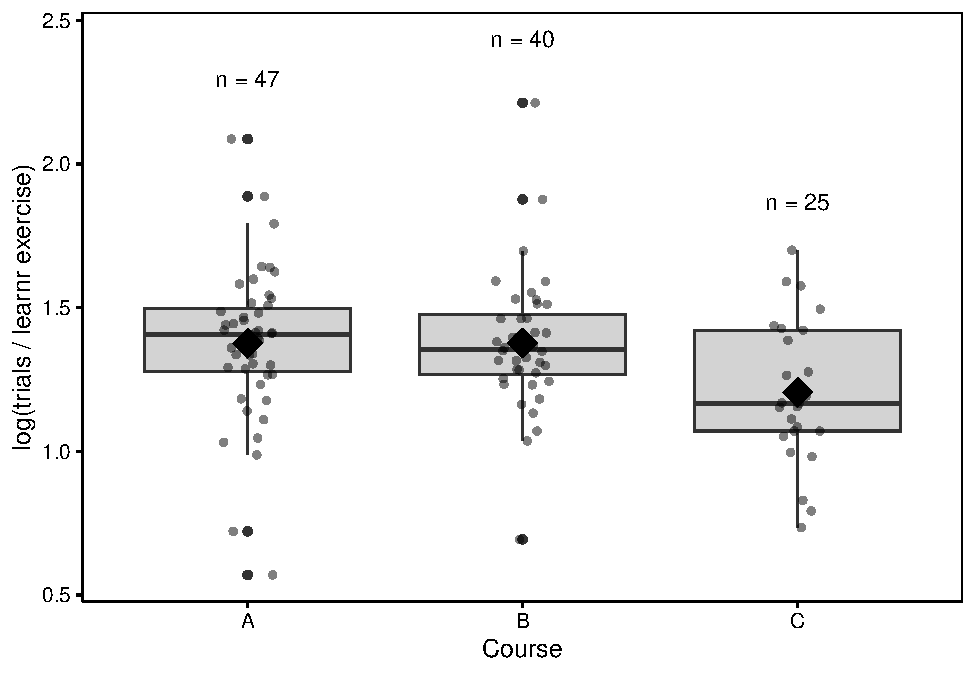
\includegraphics{teaching_data_science_files/figure-latex/fig_learn_trials-1.pdf}
\caption{Average number of retries that where required for each student
to find the right answer in learnr tutorials exercises (year 2020-2021).
This measure is used as an indirect, but objective measurement of the
cognitive workload. The black dot is the average for the whole classes
and \emph{n} is the number of observations.}
\end{figure}

{[}TODO: a paragraph describing the results + a statistical test here{]}

The perceived cognitive load required to perform these exercises is also
a key aspect. This measure the emotional state of the students after
having completed a tutorial. This has, as far as we know, not been
studied yet. We used a NASA LTX questionnaire to assess it across all
three courses. Participation to the survey was high: 48/59 (81\%), 35/45
(78\%) and 18/26 (69\%) for courses A, B, and C respectively.

\begin{figure}
\centering
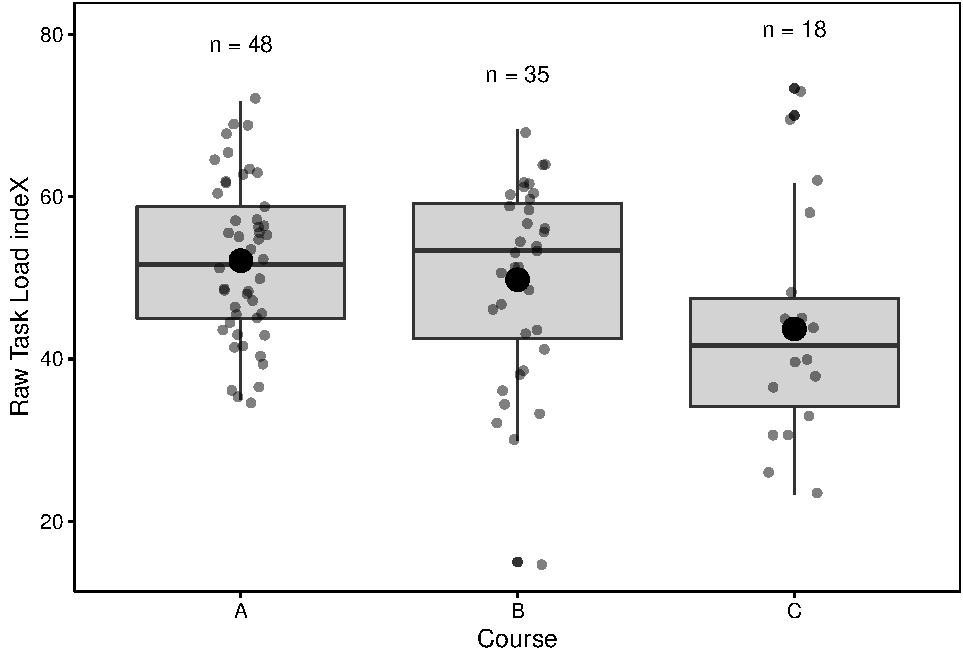
\includegraphics{teaching_data_science_files/figure-latex/fig_rtlx-1.pdf}
\caption{Perceived workload for the learnr tutorials in the three
courses (year 2020-2021). The black circle is the mean RTLX value. The
number above each box is the number of respondants.}
\end{figure}

The difficulty of the course, and thus, of the exercises in the
tutorials increase from one course to the other. However, we do not
observe an increase, neither in the number of retries, nor in the RTLX
index. On the contrary, these appear significantly lower for course C
than for course A (Tukey HSD, p-value = 0.023) TODO: INCOMPLETE
REFERENCE FOR THE TEST (MUST INDICATE ANOVA RESULTS FIRST !). The
cognitive load perceived by the students diminishes at the same time
their ability to find the right answer more rapidly. This may be a
consequence of a more fluent R coding and the better mastering of the
software environment.

\textbf{TODO: hide this output and include results in the text!}

\begin{verbatim}
## Analysis of Variance Table
## 
## Response: rtlx
##           Df  Sum Sq Mean Sq F value  Pr(>F)  
## course     2   926.9  463.47  3.5883 0.03134 *
## Residuals 98 12658.0  129.16                  
## ---
## Signif. codes:  0 '***' 0.001 '**' 0.01 '*' 0.05 '.' 0.1 ' ' 1
\end{verbatim}

\begin{verbatim}
## 
##   Simultaneous Tests for General Linear Hypotheses
## 
## Multiple Comparisons of Means: Tukey Contrasts
## 
## 
## Fit: lm(formula = rtlx ~ course, data = workload_rtlx)
## 
## Linear Hypotheses:
##            Estimate Std. Error t value Pr(>|t|)  
## B - A == 0   -2.356      2.526  -0.933   0.6183  
## C - A == 0   -8.414      3.141  -2.679   0.0228 *
## C - B == 0   -6.058      3.296  -1.838   0.1608  
## ---
## Signif. codes:  0 '***' 0.001 '**' 0.01 '*' 0.05 '.' 0.1 ' ' 1
## (Adjusted p values reported -- single-step method)
\end{verbatim}

\hypertarget{final-exam-versus-project}{%
\subsection{\texorpdfstring{Final exam \emph{versus}
project}{Final exam versus project}}\label{final-exam-versus-project}}

\begin{figure}
\centering
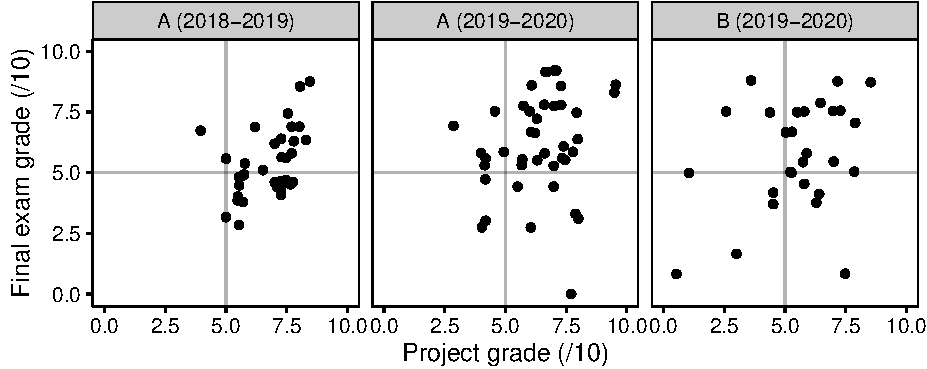
\includegraphics{teaching_data_science_files/figure-latex/fig_exams_projects-1.pdf}
\caption{Grades obtained at the final exam in function of grades
obtained for the projects for courses A and B during two years (course B
was still in its old form in 2018-2019 and is thus not represented).}
\end{figure}

In 2018-2019 and 2019-2020, the evaluation was based on the completion
of a project and on a more conventional examination at the end of the
term. The comparison of the grades obtained by each student for a
project and a final exam shows only a weak correlation between these two
types of evaluations {[}TODO: provide values here{]}. Year 2018-2019
marks the transition to a flipped classroom approach in our teaching of
these data science courses. Only one student failed in the project,
while almost one third of the same students failed their final exams.
The difficulty of the project was similar to previous years, when the
course was made of lectures followed by exercises (and when failure was
not uncommon). The flipped classroom approach leaves more time in class
to work on practical applications, to ask questions, to discuss results,
\ldots{} We hypothesize that the very low failure rate could be
explained by a better preparation to practical data analysis, but not to
the final exam.

In 2019-2020, we raised a little bit the difficulty for the project,
resulting in a more widespread distribution of the results, but with a
similar pattern showing very little correlation between the two
evaluation methods. The same conclusion can be drawn for course B, with
several students failing in one of the two evaluations, but not in the
other one.

Despite, the final examination includes a series of practical questions
(requiring to write R code to analyse data, as in the projects), this
type of assessment does not reflect the ability of the students to
correctly process and analyse biological data as well as the project.
Following these results, the final examination was abandoned for the
year 2020-2021. It is replaced by a continuous evaluation of the
students activity across all four level exercises, and especially in
individual and group projects. Results obtained with this new approach
are analysed in the following sections.

\hypertarget{students-activity-profiles-in-continuous-evaluation}{%
\subsection{Students activity profiles in continuous
evaluation}\label{students-activity-profiles-in-continuous-evaluation}}

In 2020-2021, to support the continuous evaluation method without final
exam, the course material was enriched with exercises organized into
four increasing difficulty levels, as presented in Table XXX. The
activity of the students in level 1 (H5P) and 2 (learnr) exercises is
directly recorded in a database. For the GitHub projects (levels 3 and 4
exercises), it is the git log data that are analysed. During lockdown
periods, exchange with the students and answers to their questions were
exclusively done by email, text or voice messages on Discord, either on
private or public channels. Students were allowed to freely chose their
favourite way to interact with the teachers and with each other. All
these exchanges were recorded too. Finally, records in all activities
were used to establish the final grade for the course.

Final grade is the weighted average of the scores obtained at all four
levels. The weight was adjusted from course to course according to the
importance of the different projects, mainly. To give an idea, for
course A second term, level 1 H5P exercises accounted for 5\%, 10\% for
level 2 learnr tutorials, 35\% for level 3 individual projects and 40\%
for level 4 group works. More weight is always put on projects. On
average, each student received more than 130 assessments that accounted
for the final grade. Two third of these assessments were established
manually, using evaluation grids based on the reports they write using R
Markdown {[}TODO: add a ref here{]} (.Rmd files, a literate programming
system that allows to include computations directly inside the report)
in their projects. The other third are scores automatically calculated
from the various inline exercises.

For the three courses, we recorded a total of more than 450,000 events,
which makes on average almost 3,500 events for each student. These data
contain information to characterize the behaviour and learning patterns
that the students use. They are summarized into sixteen metrics.

For H5P exercises:

\begin{itemize}
\tightlist
\item
  trials/H5P ex.: the average number of trials for each H5P exercise
  (students can retry as much as they wish and they have immediate
  feedback if their answer is correct or not),
\item
  correct H5P ex.: the fraction of H5P exercises that were correctly
  answered,
\end{itemize}

For learnr tutorial exercises:

\begin{itemize}
\tightlist
\item
  trials/learnr ex.: the average number of trials for each learnr
  exercise (here also, students can retry as much as they want),
\item
  hints/learnr ex.: in learnr exercises, students can display hints to
  help them to solve the problems (but they lose 10\% of the score of
  the exercise for each hint they view). This is the average number of
  hints per exercise that were displayed,
\item
  correct learnr ex.: the fraction of learnr exercises that were
  completed with a correct answer,
\item
  time/learnr ex.: the average time required to finish one learnr
  exercise involving R code writing.
\end{itemize}

For individual and group projects:

\begin{itemize}
\tightlist
\item
  commits / ind. projects: the average number of commits done by a
  student in one individual project,
\item
  contributions/ind. projects: the number of lines changed (added or
  subtracted) in an R Markdown report by one student in one individual
  project, on average,
\item
  commits / group projects: same as above, but for group projects,
\item
  contributions/group projects: same as above, but for group projects,
\item
  percentage of contribution to group projects: the fraction of work the
  student did, relative to all the work done in group projects (still
  only counted for .Rmd files as the number of lines changed from one
  version to the other).
\end{itemize}

For support:

\begin{itemize}
\tightlist
\item
  questions/module: the number of questions student asked in total,
  divided by the number of modules in the course,
\item
  percent of public question: the fraction of questions that the student
  posted in a public channel (a channel dedicated to the course that all
  the other students of the class can read),
\item
  contributions/question: a metric that catches the relative
  ``productivity'' of the student related to the number of questions
  they ask.
\end{itemize}

Finally, global measurements:

\begin{itemize}
\tightlist
\item
  work done: the fraction of all exercises that the student finished,
\item
  work done in time: the fraction the the exercises done in the right
  time, that is, during the proposed calendar.
\end{itemize}

{[}TODO: supplementary data: distribution of the metrics and correlation
between them{]}

A Kohonen's self-organizing map is used to create student profiles
according to their activities, see Fig. XXX. A 3x3 hexagonal cells
pattern was chosen, and students are thus classified into nine different
classes.

\begin{figure}
\centering
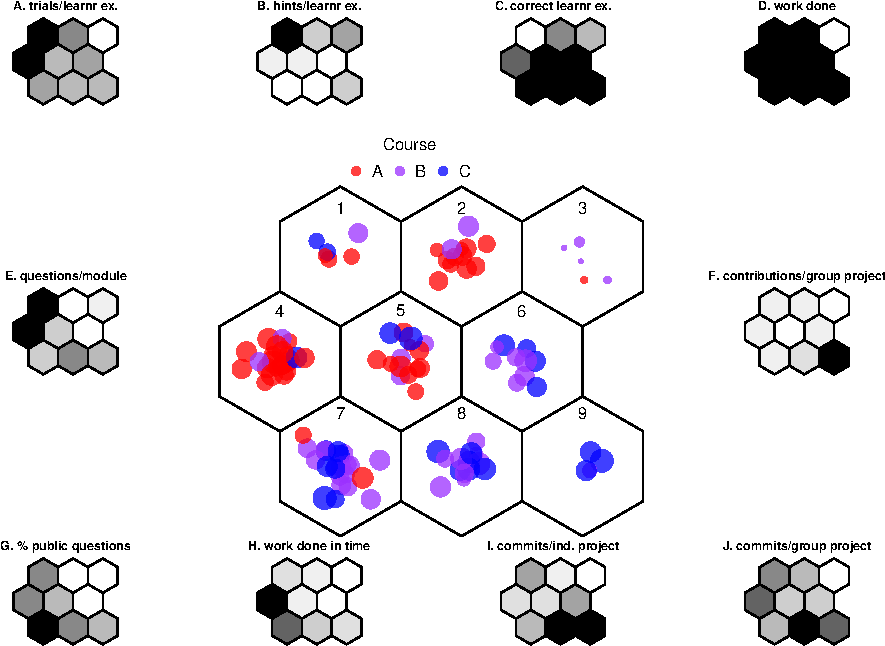
\includegraphics{teaching_data_science_files/figure-latex/fig_som-1.pdf}
\caption{Self-organizing map of the student activities across the three
courses (year 2020-2021). See the text for the explanations.}
\end{figure}

In Fig xxx, the small plots in gray show how selected metrics distribute
in the nine cells, from lowest value in white to highest value in black.
They help to decrypt the way students behave according to their profile.
Metrics that are not represented present similar patterns than others
(for instance H5P metrics exhibit a similar pattern as learnr metrics
and therefore, they are not represented). Dots in the central plot are
the various students, with colour representing the course and the
diameter of the dots representing the grade the students obtained at the
end of the course. The following paragraphs details information in that
figure. The numbers between brackets mean the cell number in the central
plot, and the upper case letters in brackets refer to the peripheral
sub-plots.

Although most students finished all, or almost all exercises (D), cell
(3) collects the few student that did only a very small part of the
exercises. These students obtained very low grades, of course. They
belong to courses A and B. On the other hand, heavy workers are at the
bottom (I \& J), and good performers in learnrs (C) are in cells (5-9).

\begin{itemize}
\item
  Besides the absent students of cell (3), cells (2 and 6) collect
  students that seldom ask questions (E), and that rarely appear on the
  public channel (G). Minor differences separate them. For instance,
  cell (2) sometimes use learnr hints (B), while cell (6) never does,
  also because they find the correct answer to the exercises more often
  by themselves (C). Asking questions is at the core of our pedagogical
  approach. So, these students do not play the game. However, they can
  possibly succeed. Some of them probably exchange with other students
  through different channels that we do not monitor. It is interesting
  to note that the cell (2) -more difficulties with learnr tutorials-
  are mainly students of course A, while cell (6) contains students of
  courses B and C. There is a clear evolution in their behaviour from
  one course to the other in term of ease in front of the exercises,
  even if they remain silent in term of teacher interactions.
\item
  Among the students that have hard time to figure out the answers to
  auto-evaluation exercises, cell (1) reassemble people that most
  heavily rely on learnr hints (B), and also are among those who need to
  retry those exercises more often before figuring out the correct
  answer (A), a characteristic they share with cell (4). These students
  also ask a lot of questions (E), both on the public and private
  channels (G, mid gray). Main difference between those two groups is
  that students in cell (4) try harder to find the answer without
  looking at the hints, while in cell (1) they give up more rapidly.
  Also these students respect the proposed schedule much more closely
  than all others (H). We have students in all courses there, but a
  majority from course A.
\item
  All these cells (1-4 plus 6) are students that exhibits sub-optimal
  behaviours in one or the other way. The remaining cells (5 \& 7-9)
  correspond to students that perform better from this point of view.
  Cell (5) has a majority of people from course A, but otherwise, also
  from course B and C. These are average actors in all categories,
  except they are fluent with level 1 (H5P, not shown) and level 2
  (learnr, C) exercises.
\item
  Moving from cell (5) to (7), (8) and (9), we encounter increasingly
  top performers. The number of students from course A becomes
  progressively lower, while course B, and especially C dominate in
  these groups. Cell (7) use largely the public channel (G) and respect
  the schedule quite well (H) as main difference from those from cell
  (5). Students in cells (8) and (9) are not so much in time, but this
  is because they are heavier workers in the projects, both in the
  individuals (I) and in the groups (J) activities. This needs obviously
  more time. In cell (9) we have also the students that contributes the
  most to the reports in term of lines added or deleted (F).
\end{itemize}

In overall, at the top of the SOM, cells (1-4, plus 6) contain students
with not optimal behaviour, cell (5) are average students, and cells
(7-9) at the bottom exhibit profiles corresponding to best performers.
The pattern is also visible between courses A (mainly distributed at the
top or centre) to B and C (more represented at the bottom). This
suggests that students need time to get used to the course, its
pedagogical approach, and/or the software environment they have to use.

\hypertarget{transition-between-face-to-face-and-distance-learning}{%
\subsection{Transition between face-to-face and distance
learning}\label{transition-between-face-to-face-and-distance-learning}}

Due to Covid-19 lockdown periods, distance learning had to be adopted
abruptly. We analyse the activity collected during academic years
2019-2020 and 2020-2021 to assess the impact of these transition on the
progression of the students (contributions they make to the projects per
time unit). One academic term is divided here into seven work periods of
approximately two weeks (remind that it is the rhythm of the courses:
one module every second week). The classes of the second term of the
year 2019-2020 start at period Y1P09, since period Y1P08 is reserved for
the exams. The courses of the first term of 2020-2021 begins at Y2P01.
First lockdown started at period Y1P11 for one month and an half. Second
lockdown stared at Y2P03 and lasted at then end of the second term
(Y2P15). During the first lockdown, we rapidly opened the dedicated
Discord channels and a common email address for all teachers was
installed for a faster reaction.

\begin{figure}
\centering
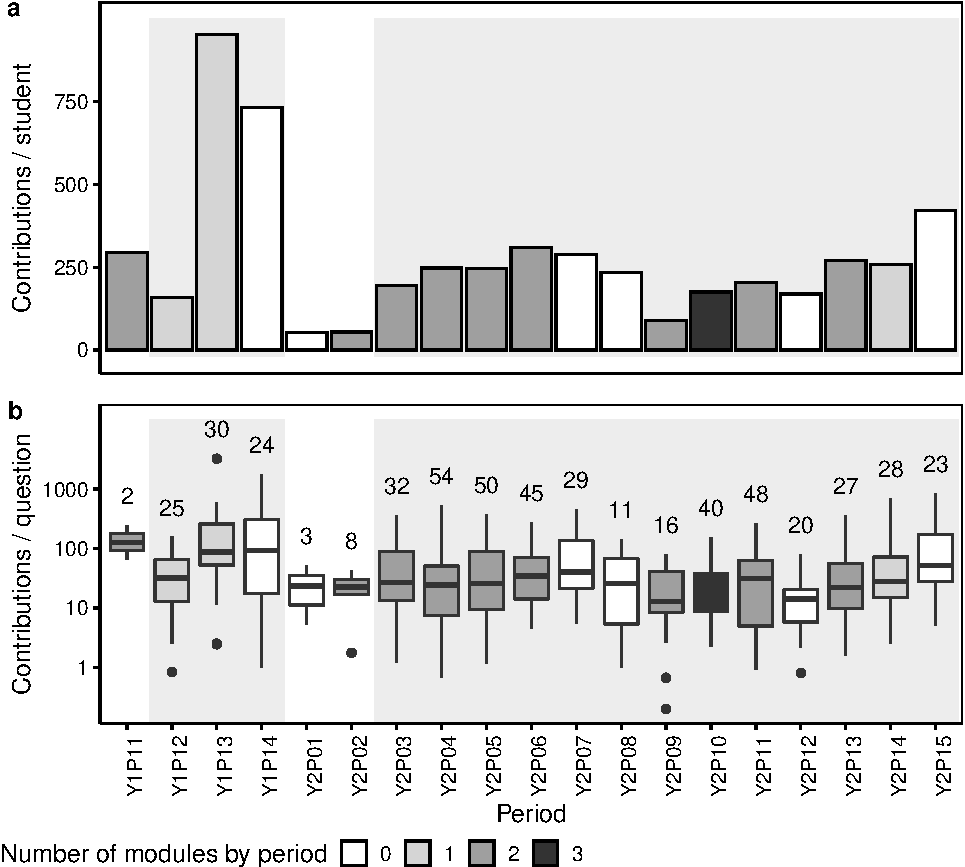
\includegraphics{teaching_data_science_files/figure-latex/fig_support_by_time-1.pdf}
\caption{a. Contributions of the students to the projects by periods of
two weeks of course. b. Contributions by question asked (log scale) as a
proxy measurement of the effect of student-teacher interactions on the
progression in data analysis. Light gray background indicates periods
where distance teaching was mandatory due to Covid-19 lockdown (Y1 is
2019-2020, Y2 is 2020-2021).}
\end{figure}

{[}TODO: this paragraph must be adapted and reworked!{]} The
contributions to the reports remains relatively proportional to the
number of questions the students sent by email or Discord messages, no
matter the period and the intensity of the work as indicated by the
number of modules to be completed during the period, all three courses
pooled together. Only the number of students that ask questions by there
channels change between face-to-face and distance teaching (much less in
face-to-face because most of the students ask their questions directly
in the classroom). Transition from direct interaction to electronic
exchange was quasi immediate during lockdown. Consequently, support
provided by the teachers in distance learning \ldots{} to be continued.

\hypertarget{discussion}{%
\section{Discussion}\label{discussion}}

{[}juste quelques idées\ldots{} à développer et à traduire en anglais
bien sûr.{]}

\begin{itemize}
\item
  la charge cognitive mesurée et perçue dans les tutoriels learnrs
  diminue pour le cours C alors même que c'est le plus difficile.
  Discussion sur le long temps qu'il faut aux étudiants (4 semestres)
  pour devenir à l'aise avec l'environnment logiciel et les concepts de
  base en science des données. A l'avenir, nous pourrons utiliser ces
  points de référence (index RTLX) pour encore améliorer ces tutoriels
  de ce point de vue.
\item
  L'examen en fin de période, même s'il reprend des questions liées à de
  la pratique et de l'utilisation d'outils, ne mène pas à une évaluation
  fortement corrélée avec l'activité qui nous intéresse le plus, à
  savoir, la capacité de l'étudiant à analyser des données billogiques
  réelles. Cette capacité est parfaitement évaluée dans les projets de
  niveau 1, et surtout de niveau 2 qui correspondent très précisément à
  une telle activité. Par conséquent, l'évaluation ne se fait plus via
  un examen final, mais uniquement via les prestations des étudiants
  dans les projets, ainsi que (pour une part relativement faible de 15\%
  de la note finale), leur progression dans l'apprentissage de la
  matière via la réalisation des exercises de niveau 1 et des tutoriels
  de niveau 2, ceci afin de les encourager à réaliser complètement tous
  les exercises et à les faire dans l'ordre croissant de difficulté.
\item
  Même au sein d'une cohorte d'étudiants ayant un parcours académique
  similaire, nous notons de très grosses différences de stratégie dans
  les activités d'apprentissage. Si plusieurs stratégies différentes
  sont associées à une acquisition bonne à erxcellente des compétences
  telle qu'attestée par les notes obtenues, plusieurs profils sont
  systématiquement associés à des performances faibles. Nous espérons
  que les profils ainsi établis via cartes auto-adaptatives permettront
  à l'avenir de détecter plus tôt les étudiants à suivre plus
  particulièrement et à réfléchir à des approches alternatives pour eux
  afin de les aider (pédagogie inclusive).
\item
  Les études portant sur le changements d'attitudes au sein de semestre
  ne montre pas différence significative. La comparaison entre les 3
  cours met en avant qu'il faut plusieurs cours en continu afin
  d'observer une changement de la charge cognitive des étudiants.
\item
  Apprentissage en continu sur 3 années successives (cohérence entre le
  programme et l'approche pédagogique), les résultats sont meilleurs
  vers la 3ème années.
\item
  Pendant les périodes de confinements, le passage brutal à des cours en
  présentiel vers des cours en distaznciel nécesite une période
  d'adaptation que nous avons quantifié dans notre cas à environ 2
  semaine. Il s'agit ici du temps d'adaptation des étudiants, sachant
  que du côté des enseignants, nous avons réagit immédiatement (et même
  anticipé) en mettant en place très rapidement les canaux de
  communication alternatifs via le mail et Discord.
\end{itemize}

\hypertarget{conclusions}{%
\section{Conclusions}\label{conclusions}}

\begin{itemize}
\item
  Exam classique évalue mal la capacité d'evaluer des données
  biologiques par eux même
\item
  Les biologistes non expert de l'informatique est une challenge vu le
  nombre important de notions a apprendre utilisation d'un ordi, gestion
  de projet, statistique. Il faut décomposer ces notions en petites
  étapes successives si nous ne voulons pas les perdre rapidement. Notre
  approche en 3 cours étalés sur 5 quadrimestres successifs et étalés
  sur 3 années semblent correspondre à un bon timing pour ce type
  d'étudiant qui, au départ, n'a aucune notion de statistique, et très
  peu de connaissance des outils des logiciels couramment utilisées par
  le scientifique des données.
\item
  Néanmoins, malgré leur habituation progressive, ces logiciels restent
  vus comme pointu et diffficile d'utilisation (SUS) {[}à voir si on met
  cela dans l'article: on a déjà beaucoup ! =\textgreater{} réserver
  cela pour un autre article l'annéde prochaine peut-être ?{]}.
\item
  l'evaluation continue et l'analyse de projet via des grilles critérié
  semble une approche intéressante pour juger de la capacité des
  étudiant à bosser {[}on a pas développé cela au final, il me
  semble{]}.
\item
  la catégorisation des étudiants en différents profils d'apprenants
  ayant adopté des stratégies très contrastées démontre une grande
  diversité des apprenants, même à l'intérieur d'un groupe a priori
  homogène (n,ous ne nous trouvons pas ici dans une grande classe qui
  regrouperait des étudiants d'horizons très différents comme les cours
  d'introduction à la science des données tels que pratiques dans
  certaines grandes universités américaines). Ceci est un premier pas
  vers une pédagogie différencié et plus inclusive qui s'avèrent être
  des éléments importants ici.
\end{itemize}

\hypertarget{references}{%
\section*{References}\label{references}}
\addcontentsline{toc}{section}{References}

\hypertarget{refs}{}
\begin{CSLReferences}{1}{0}
\leavevmode\hypertarget{ref-Auker2020}{}%
Auker, Linda A., and Erika L. Barthelmess. 2020. {``{Teaching R in the
undergraduate ecology classroom: approaches, lessons learned, and
recommendations}.''} \emph{Ecosphere} 11 (4): e03060.
https://doi.org/\url{https://doi.org/10.1002/ecs2.3060}.

\leavevmode\hypertarget{ref-Baker2016}{}%
Baker, Monya. 2016. {``1,500 Scientists Lift the Lid on
Reproducibility.''} \emph{Nature} 533 (7604): 452--54.
\url{https://doi.org/10.1038/533452a}.

\leavevmode\hypertarget{ref-Banks2019}{}%
Banks, George C., James G. Field, Frederick L. Oswald, Ernest H.
O'Boyle, Ronald S. Landis, Deborah E. Rupp, and Steven G. Rogelberg.
2019. {``{Answers to 18 Questions About Open Science Practices}.''}
\emph{Journal of Business and Psychology} 34 (3): 257--70.
\url{https://doi.org/10.1007/s10869-018-9547-8}.

\leavevmode\hypertarget{ref-Baumer2014}{}%
Baumer, Ben, Mine Cetinkaya-Rundel, Andrew Bray, Linda Loi, and Nicholas
J. Horton. 2014. {``{R Markdown: Integrating A Reproducible Analysis
Tool into Introductory Statistics}.''} \emph{Technology Innovations in
Statistics Education} 8 (1). \url{https://doi.org/10.5070/t581020118}.

\leavevmode\hypertarget{ref-Boettiger2015}{}%
Boettiger, Carl. 2015. {``{An Introduction to Docker for Reproducible
Research}.''} \emph{SIGOPS Oper. Syst. Rev.} 49 (1): 71--79.
\url{https://doi.org/10.1145/2723872.2723882}.

\leavevmode\hypertarget{ref-Byers1989}{}%
Byers, J C, A Bittner, and S Hill. 1989. {``{Traditional and raw task
load index (TLX) correlations: Are paired comparisons necessary? In
A}.''} In.

\leavevmode\hypertarget{ref-Cetinkaya-Rundel2021}{}%
Çetinkaya-Rundel, Mine, and Victoria Ellison. 2021. {``{A Fresh Look at
Introductory Data Science}.''} \emph{Journal of Statistics Education} 0
(0): 1--27. \url{https://doi.org/10.1080/10691898.2020.1804497}.

\leavevmode\hypertarget{ref-Cetinkaya-Rundel2018}{}%
Çetinkaya-Rundel, Mine, and Colin Rundel. 2018. {``{Infrastructure and
Tools for Teaching Computing Throughout the Statistical Curriculum}.''}
\emph{American Statistician} 72 (1): 58--65.
\url{https://doi.org/10.1080/00031305.2017.1397549}.

\leavevmode\hypertarget{ref-Donoho2017}{}%
Donoho, David. 2017. {``{50 Years of Data Science}.''} \emph{Journal of
Computational and Graphical Statistics} 26 (4): 745--66.
\url{https://doi.org/10.1080/10618600.2017.1384734}.

\leavevmode\hypertarget{ref-Estrellado2020}{}%
Estrellado, Ryan A., Emily A. Bovee, Jesse Mostipak, Joshua M.
Rosenberg, and Isabella C. Velásquez. 2020. \emph{{Data science in
education using R}}. London, England: Routledge.
\url{https://datascienceineducation.com/}.

\leavevmode\hypertarget{ref-Fiksel2019}{}%
Fiksel, Jacob, Leah R. Jager, Johannna S. Johanna S Hardin, and Margaret
A. Taub. 2019. {``{Using GitHub Classroom To Teach Statistics}.''}
\emph{Journal of Statistics Education} 27 (2): 110--19.
\url{https://doi.org/10.1080/10691898.2019.1617089}.

\leavevmode\hypertarget{ref-Freeman2014}{}%
Freeman, Scott, Sarah L. Eddy, Miles McDonough, Michelle K. Smith,
Nnadozie Okoroafor, Hannah Jordt, and Mary Pat Wenderoth. 2014.
{``{Active learning increases student performance in science,
engineering, and mathematics}.''} \emph{Proceedings of the National
Academy of Sciences} 111 (23): 8410--15.
\url{https://doi.org/10.1073/PNAS.1319030111}.

\leavevmode\hypertarget{ref-Hart1988}{}%
Hart, Sandra G., and Lowell E. Staveland. 1988. {``{Development of
NASA-TLX (Task Load Index): Results of Empirical and Theoretical
Research}.''} \emph{Advances in Psychology} 52 (C): 139--83.
\url{https://doi.org/10.1016/S0166-4115(08)62386-9}.

\leavevmode\hypertarget{ref-Hsing2019}{}%
Hsing, Courtney, and Vanessa Gennarelli. 2019. {``{Using GitHub in the
Classroom Predicts Student Learning Outcomes and Classroom Experiences:
Findings from a Survey of Students and Teachers}.''} In
\emph{Proceedings of the 50th ACM Technical Symposium on Computer
Science Education}, 672--78. SIGCSE '19. New York, NY, USA: Association
for Computing Machinery. \url{https://doi.org/10.1145/3287324.3287460}.

\leavevmode\hypertarget{ref-Krathwohl2002}{}%
Krathwohl, David R. 2002. {``{A Revision of Bloom' s Taxonomy: An
otherview}.''} \emph{Theory Into Practice} 41 (4): 212--18.
\url{https://doi.org/10.1207/s15430421tip4104}.

\leavevmode\hypertarget{ref-Larwin2011}{}%
Larwin, Karen, and David Larwin. 2011. {``{A meta-analysis examining the
impact of computer-assisted instruction on postsecondary statistics
education: 40 years of research}.''} \emph{Journal of Research on
Technology in Education} 43 (3): 253--78.
\url{https://doi.org/10.1080/15391523.2011.10782572}.

\leavevmode\hypertarget{ref-Marx2013}{}%
Marx, Vivien. 2013. {``{The big challenges of big data}.''}
\emph{Nature} 498 (7453): 255--60.
\url{https://doi.org/10.1038/498255a}.

\leavevmode\hypertarget{ref-Onwuegbuzie2003}{}%
Onwuegbuzie, Anthony J., and Vicki A. Wilson. 2003. {``{Statistics
Anxiety: Nature, etiology, antecedents, effects, and treatments--a
comprehensive review of the literature}.''} \emph{Teaching in Higher
Education} 8 (2): 195--209.
\url{https://doi.org/10.1080/1356251032000052447}.

\end{CSLReferences}

\end{document}
